There are three types of requests that will be processed by the application: single flight, round trip and multi-city trip. A user must initially select the desired type of search, and follow this with the completion of a series of forms that collect the relevant input. 

Every request requires at least an origin and a destination, as well as a start date. There are other search attributes which might be relevant, according to the selected trip type, and the duration associated to each city that will be visited. A complete list of the input that may be collected from the user is presented in table \ref{table:input_action_reducer} (left column). 


\begin{table}[htpb]
  \centering
  \caption{Parallelism between User Input, Actions and Reducers. To each user defined input corresponds an 
  action, declaring the intent of changing the state with some specific data, and a reducer, which actually modifies the state. }
  \setlength{\tabcolsep}{8mm}
  \label{table:input_action_reducer}
  \begin{tabular}{ccc}
  \hline
  \\[-0.75em]
  User input  & Action               & Reducer                    \\ \hline
  \\[-0.75em]
  origin      & actOrigin(origin)    & setOrigin(state, action)   \\
  \\[-0.75em]
  destination & actDest(dest, index) & setDest(state, action)     \\
  \\[-0.75em]
  duration    & actDur(dur, index)   & setDuration(state, action)     \\
  \\[-0.75em]
  start date  & actDate(date, index) & setStartDate(state, action)     \\
  \\[-0.75em]
  submit      & actRequest(request)  & setResponse(state, action) \\ \hline
  \end{tabular}
\end{table}


Then, to every user input it is associated an action and a reducer. Table \ref{table:input_action_reducer} also defines the action that is dispatched each time the input is updated (center column), and the corresponding reducer that is responsible for updating the state of the application (right column). Note that the last user input (\textit{submit}) is processed by an asynchronous action. Thus, after the submission of the request, the reducer will be called only upon receiving the response from the SSA, updating the state by storing the received data, and triggering the update of the user interface. 

The developed application forces the user to submit the request, by clicking on a button that dispatches an action. During the development of the application, the possibility of removing this button, and to automatically dispatch a request was considered. However, it was subsequently rejected because of the difficulty to know if a certain request is complete. For example, given a single flight request, knowing if the request is complete is simply a matter of verifying if an origin, destination and departure date exist. For a round-trip, the duration would also be a requirement. However, for multicity requests, unless the user specifies how many cities are to be visited, there is no way of knowing when a request is complete. Furthermore, any change to an already complete request would trigger another new request. Thus, it must be an user defined action to declare the intention of submitting a request.


%_________________ INPUT FLOW ______________

% \begin{figure}[H]
%   \centering
%   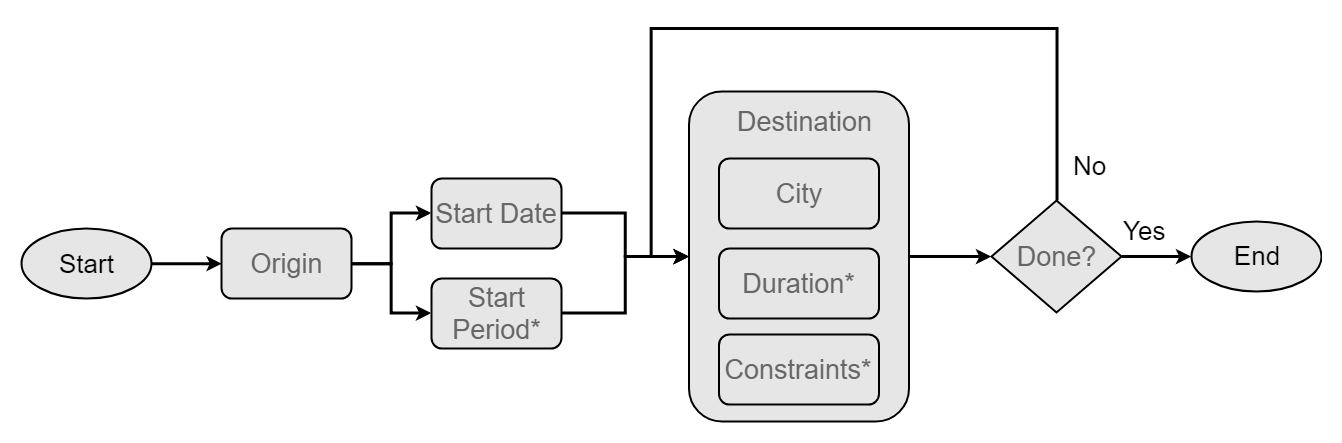
\includegraphics[width=\textwidth]{Figures/system_implementation/user_input.png}
%   \caption{Block diagram of the user input cycle.}
%   \label{fig:user_input}  
% \end{figure}


%_________________ AIRPORT VALIDATION ______________

% Figure of airport validation.
% This is not a central key to the program, so use the image only if we need extra content
% \begin{figure}[H]
%   \centering
%   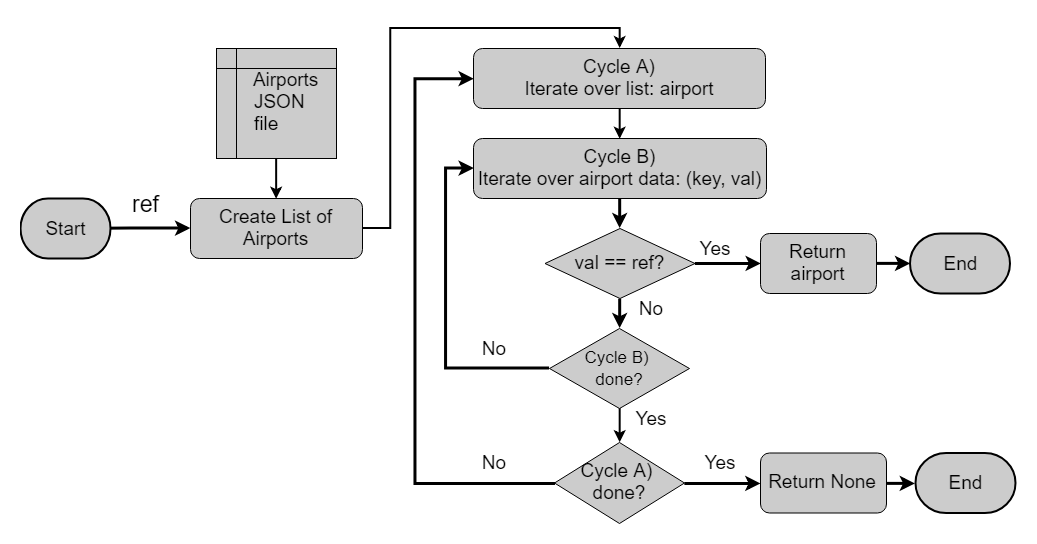
\includegraphics[width=\textwidth]{Figures/system_implementation/airports.png}
%   \caption{Validation of an user introduced airport based on an airport list stored in a JSON file.}
%   \label{fig:airports}  
% \end{figure}